\documentclass{class/technicalReportUAB}
\usepackage{booktabs}
\usepackage{todonotes}

\graphicspath{{./figures/}{./figures/png/}}

%%%%%%%%%%%%%%%%%%%%%%%%%%%%%%%%%%%%%%%%%%%%%%%%%%%%%%%%%%%%%%%%%%%%%%%%%%
% Template configuration
%%%%%%%%%%%%%%%%%%%%%%%%%%%%%%%%%%%%%%%%%%%%%%%%%%%%%%%%%%%%%%%%%%%%%%%%%%

\renewcommand{\externalOrganization}{}
\renewcommand{\externalProjectReference}{Retos Colaboración RTC2019-007434-7}
\renewcommand{\internalProjectReference}{RTC2020}
\renewcommand{\reportReferenceAffix}{D1} % e.g., R0 for the first report
\renewcommand{\reportReference}{\internalProjectReference-\reportReferenceAffix}

\renewcommand{\documentTypeName}{Technical Report}
\renewcommand{\documentVersion}{1}
\renewcommand{\documentTitle}{Final performance evaluation}
\renewcommand{\pdfTitle}{\documentTitle\ --- [\pdfAuthor]}
\renewcommand{\pdfAuthor}{UAB - GICI}
\renewcommand{\documentSubtitle}{Project: \externalOrganization\ \externalProjectReference\\}
\renewcommand{\documentDate}{\today}
\renewcommand{\documentReference}{\reportReference}
\renewcommand{\documentAbstract}{
A compression system has been developed as a part of the Retos Colaboración RTC2019-007434-7 project.
This technical report describes its main features and configurable parameters, analyzing the impact
on compression performance and execution time. 
A comparison with JPEG~2000, JPEG-LS and CCSDS~123.0-B-2 is also provided. Results indicate that 
the developed system provides the best compression vs. execution time trade-offs in the near-lossless regime, being significantly 
faster than all other tested alternatives that allow controlling the peak absolute error of the reconstructed samples.
}

%% Page format can be adapted as needed
% 
% \renewcommand{\leftHeaderContents}{%
% \textbf{\documentTitle}\\\documentTypeName\\\externalProjectReference
% }
% 
% \renewcommand{\rightHeaderContents}{%
% Updated: \documentDate \\
% \documentReference\\
% Document version: v\documentVersion
% }
% 
% \renewcommand{\leftFooterContents}{%
% \externalProjectReference\ -- \documentReference\ -- v\documentVersion
% }

%%%%%%%%%%%%%%%%%%%%%%%%%%%%%%%%%%%%%%%%%%%%%%%%%%%%%%%%%%%%%%%%%%%%%%%%%%

\usepackage{hyperref}
\hypersetup{
    pdftitle = {\pdfTitle},
    pdfauthor = {\pdfAuthor}
}

\begin{document}

\coverpage

\newpage

\section{Introduction}

This technical report presents a summary of the performance attained by the variable-to-fixed (V2F) codec developed
by the GICI group (\url{gici.uab.cat}) of the Universitat Autònoma de Barcelona 
as a part of the Retos Colaboración project with reference RTC2019-007434-7.

The V2F codec is based on an entropy coding stage that iteratively processes one or more consecutive input samples and encodes them as a 
single, fixed-length compressed word. This process is guided by the structure of the selected \textit{code forest}, which can be 
built for any sample value distribution.
This V2F entropy coder can be very efficiently implemented in software that does not require bit mangling nor if-else branches.
To accompany the entropy coding stage, a set of best-effort decorrelation functions are made available, as well as a quantization stage that allows
trading better coding efficiency for a controlled amount of distortion in the reconstructed images.

This codec, as well as its side utilities, prebuilt code forests, evaluation scripts, and full documentation
are available as an open-source project at \mbox{\url{github.com/gici-uab/v2f_codec}}.
% 
Other intermediate reports, including an analysis of relevant works in the state of the art and other studies
produced during the development of this codec are available at \mbox{\url{github.com/gici-uab/v2f_codec/tree/master/reports}}.

Section~\ref{sec:test_corpora} provides a description of the test corpora employed for the design and evaluation of the V2F codec.
Sections~\ref{sec:lossless_results} and~\ref{sec:lossy_results} analyze respectively the lossless and lossy compression capabilities 
of the codec. Two coding strategies evaluated and ultimately discarded during the codec design process are described in Section~\ref{sec:discarded}.
Finally, Section~\ref{sec:conclusions} summarizes the main conclusions of this report. Note that most figures have been moved 
to Appendix~\ref{sec:figures} to enhance readability.


\section{Test corpora}\label{sec:test_corpora}

Three test corpora have been considered in this report: 
\begin{itemize}
\item \textit{fields2020}: 160 images
\item \textit{boats2020}: 12 images
\item \textit{newsat2022}: 248 images
\end{itemize}
All of them consist of L0, 8-bit grayscale images of size 5120$\times$5120 provided by the Satellogic Earth Observation company (\url{satellogic.com}).
Each image contains 4 horizontal regions, each depicting a different part of the spectrum, similar to the following example:

\begin{center}
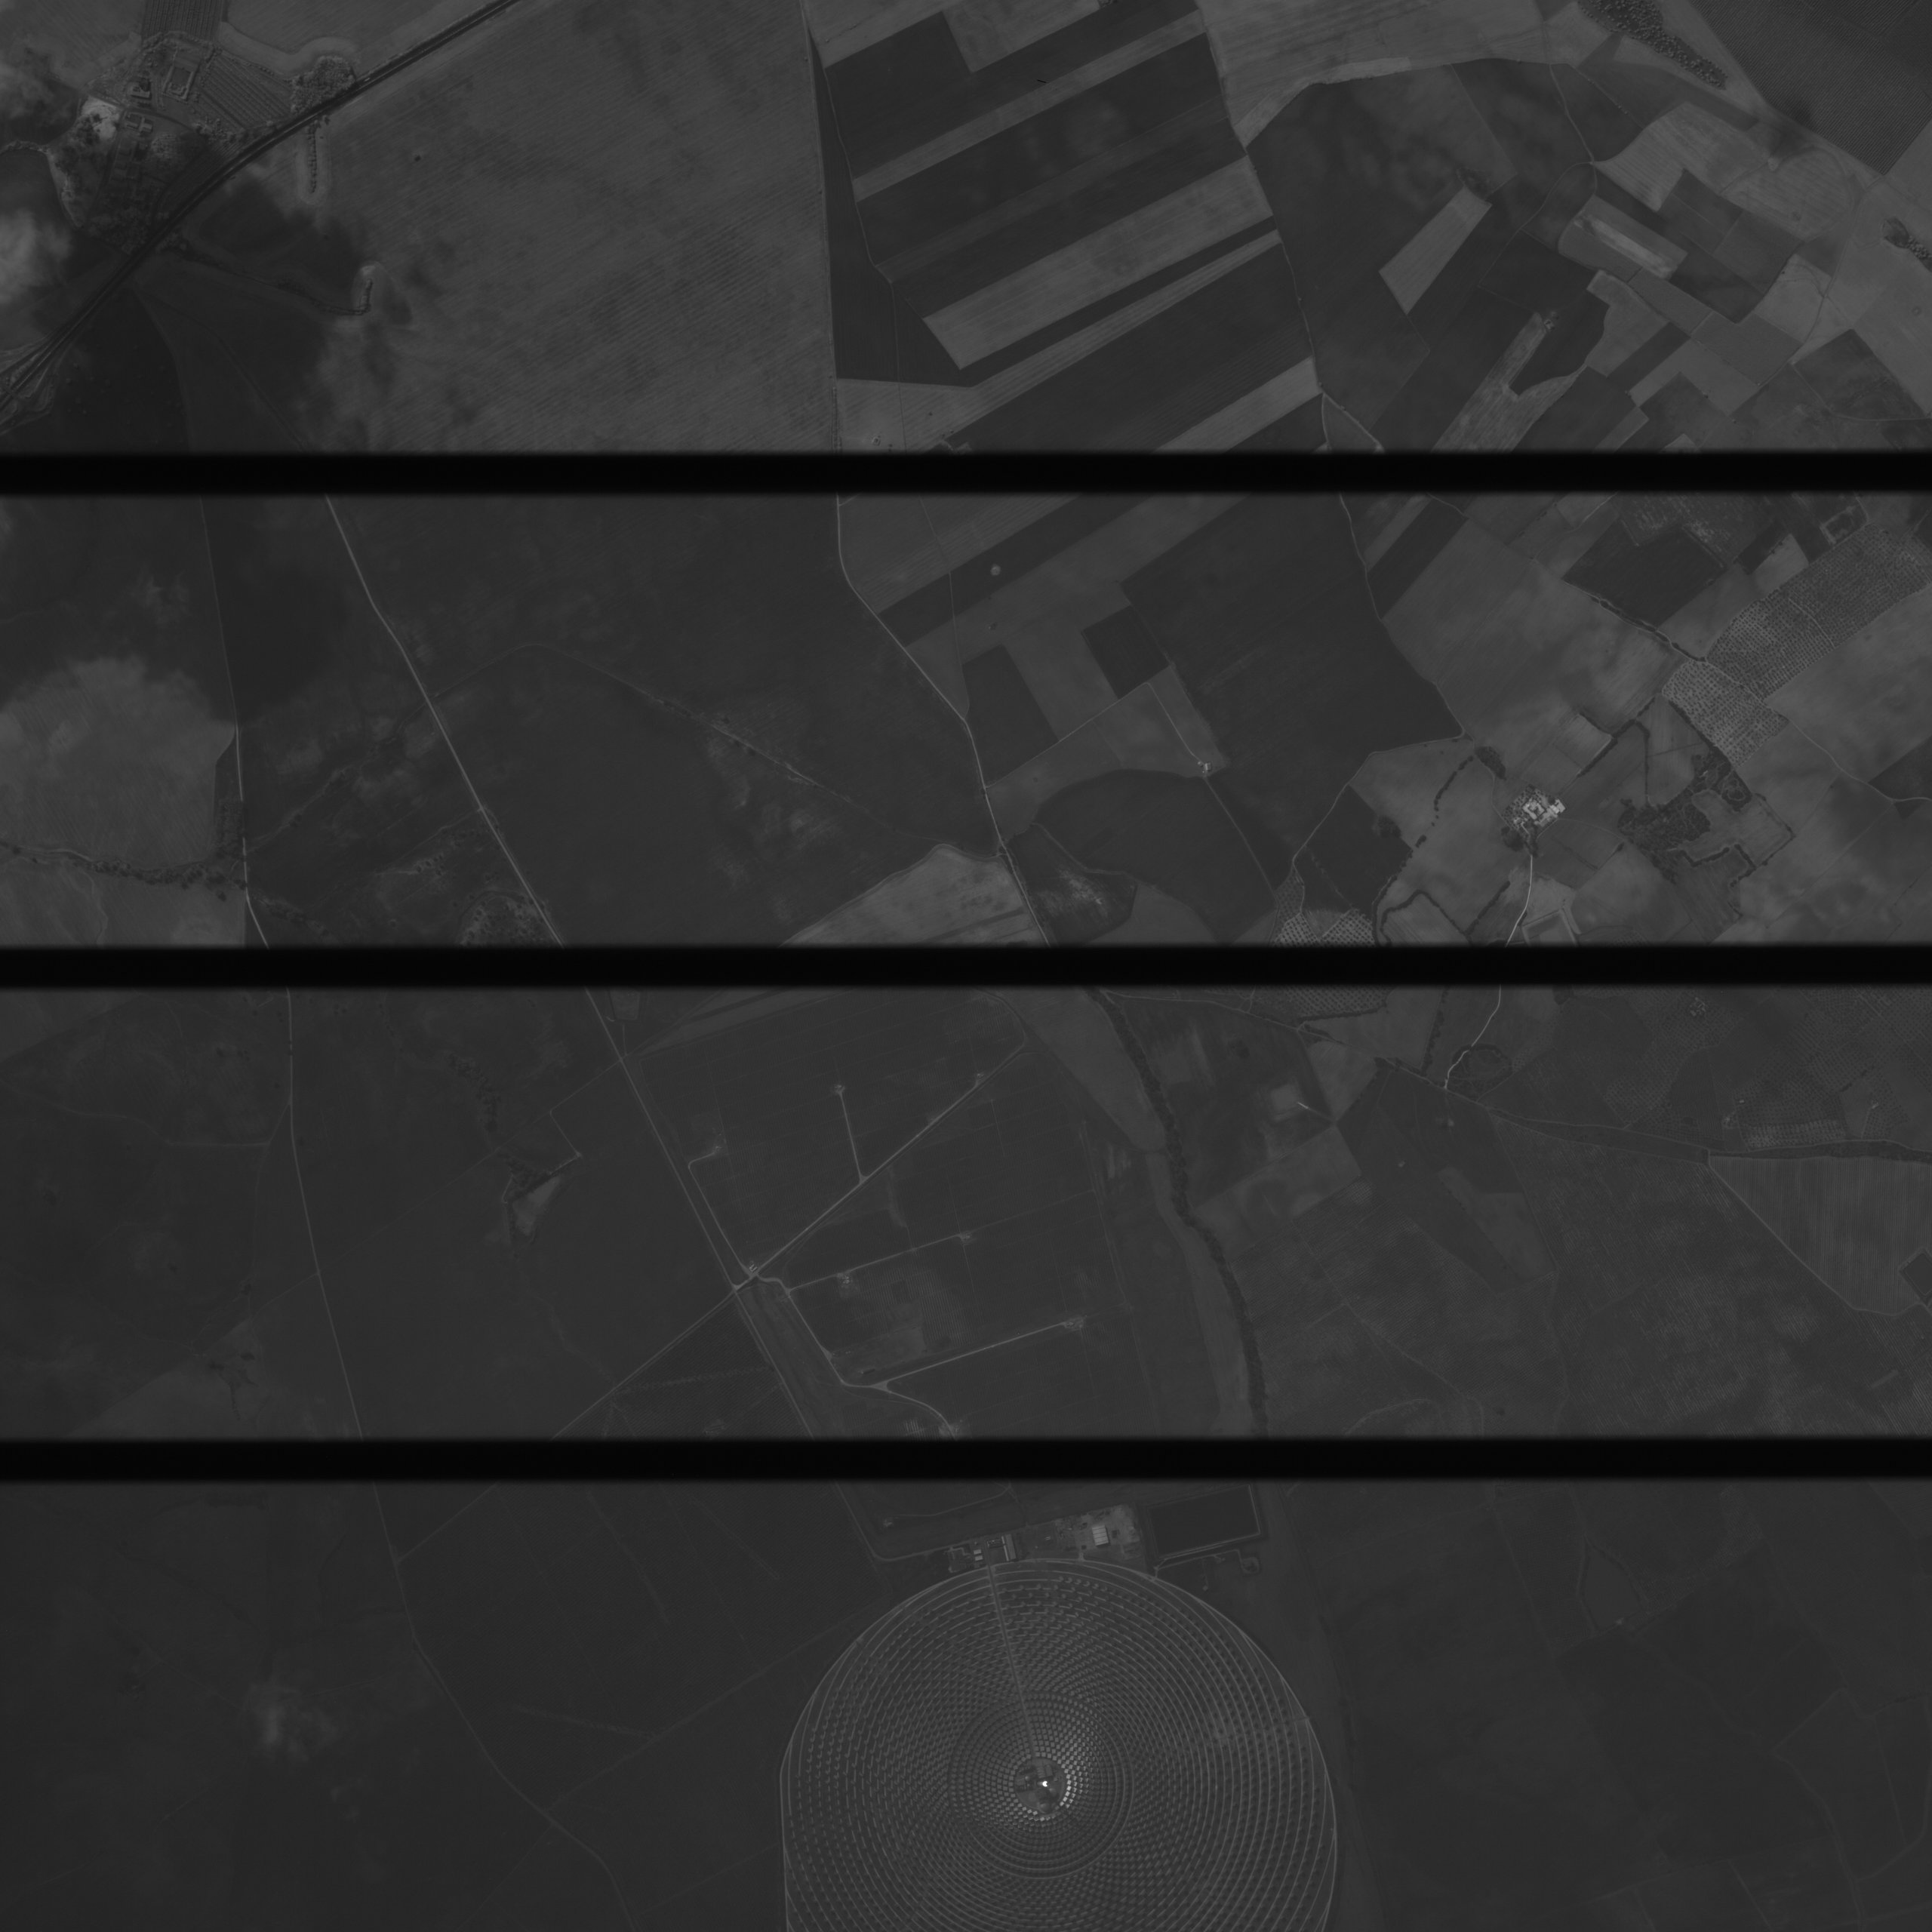
\includegraphics[width=0.5\linewidth]{./plots/dataset_analysis/corpus_sample.png}
\end{center}

Development of the V2F codec has been performed based on the analysis of the \textit{fields2020} and \textit{boats2020} corpora.
In particular, the training of the prebuilt code forests has been based on the statistical properties of these two sets.
The third corpus, \textit{newsat2022} is employed only to evaluate the coding efficiency of the developed codec.

Several properties of these corpora have been analyzed and are shown next. 
% 
Fig.~\ref{fig:sample_distribution} displays average sample distributions of the original images. These are comparable
to natural images, save for the spike between around value 10, due to the shadow areas that divide the horizontal regions of the images.
% 
Zero-order entropies are shown in Fig.~\ref{fig:entropy}. These range between 5 and 7 bits per sample (bpppc), out of the maximum 8~bpppc
possible in 8-bit images.

\section{Lossless compression results}\label{sec:lossless_results}

The lossless compression performance of the developed V2F codec is evaluated in this section and compared to some of the most relevant contending algorithms.
% 
Several parameters available in the V2F prototype have been evaluated:
\begin{itemize}
 \item Number of trees in each coding forest. More trees allow a more precise representation of the training data's distribution, at the cost of a larger
       memory footprint and decreased coding efficiency.
 \item The prediction mode used for decorrelation. Four best-effort predictors have been implemented:
    \begin{itemize}
    \item W: predict each pixel with the value of the previous one.
    \item (W1 + W2)/2: predict each pixel with the average of the two previous ones.
    \item JPEGLS: predict each pixel using the same logic as the JPEG-LS algorithm (see \url{https://en.wikipedia.org/wiki/Lossless_JPEG#Decorrelation/prediction} for details)
    \item FGIJ: predict each pixel as the average of four neighbors. These are the two pixels to the left, the pixel above, and the pixel above and left of the predicted sample.
    \end{itemize}
 \item Compression or not of the shadow regions between the horizontal data regions. The \textit{noshadow} label is used to indicate that these shadows are not compressed,
       and are then reconstructed to values identically zero.
\end{itemize}
% 
The remaining compressors included in this comparison are:
\begin{itemize}
 \item Kakadu JPEG~2000 (\url{kakadusoftware.com}) (run in a single thread, i.e., without employing parallelism)
 \item JPEG-LS (\url{https://jpeg.org/jpegls/index.html})
 \item The CCSDS 123.0-B-2 standard (\url{https://public.ccsds.org/Publications/BlueBooks.aspx}), using the French space agency (CNES)
       implementation available at \url{https://logiciels.cnes.fr/en/license/173/749}.
\end{itemize}

The average lossless compression bitrates across all test corpora are shown for each codec and V2F configuration in Fig.~\ref{fig:lossless_bpppc}.
The compression efficiency of the three non-V2F algorithms is superior to that of configurations of the V2F codec. Notwithstanding, this performance
gap can be reduced below 0.2~bps for the FGIJ predictor, no shadow coding and more than 1 tree in the code forest.
It should be noted that the FGIJ predictor consistently produces the best V2F coding performance given a number of code forest trees and 
whether shadows are compressed (true lossless) or not (lossless outside the shadow regions).
% 
Lossless compression results for a selection of V2F configurations are shown for each of the tree test corpora separately in Figs.~\ref{fig:lossless_bpppc_fields},
~\ref{fig:lossless_bpppc_boats} and~\ref{fig:lossless_bpppc_newsat}. As can be observed, the relative efficiency of all codecs is similar
in spite of the fact that V2F code forests are trained using only data from two of the three test corpora.


An estimation of the time complexity of each compression algorithm and V2F configuration is shown in Fig.~\ref{fig:lossless_time}. 
All V2F configurations are significantly faster than JPEG-LS and CCSDS 123.0-B-2, sometimes over twice as fast.
The Kakadu JPEG~2000 codec exhibits speeds comparable (but slightly slower) than the fastest V2F codecs.
% 
It must be highlighted that these results are obtained in hardware not representative of that available in space
(an Intel(R) Core(TM) i7-8700 CPU @ 3.20GHz was used to generate Fig.~\ref{fig:lossless_time}). Furthermore, unlike Kakadu JPEG~2000, 
no special assembly instructions have been used to speed up the V2F codec prototype.

\section{Lossy compression results}\label{sec:lossy_results}

Lossy compression results are shown for a selection of V2F configurations, as well as for the aforementioned JPEG~2000, JPEG-LS and CCSDS 123.0-B-2 implementations.
% 
All these algorithms except for JPEG~2000 compress in a near-lossless regime, i.e., bounding the peak absolute error (PAE) of the reconstructed samples.
In particular, the V2F codecs perform a quantization stage before prediction to minimize the computational workload.
On the other hand, the JPEG~2000 standard is designed to maximize the peak signal-to-noise ratio (PSNR), without any guarantee in terms of PAE.

The average PSNR, PAE and compression time results as a function of the obtained compressed data rate are shown in Figs.~\ref{fig:lossy_psnr}, ~\ref{fig:lossy_pae} and~\ref{fig:lossy_time},
respectively. In terms of PSNR, the V2F codecs produce competitive albeit lower fidelity at all tested compressed data rates. 
When the PAE is considered, the V2F codecs provide lower coding efficiency than JPEG-LS and CCSDS 123.0-B-2, although in most cases at a fraction of the execution time.
In turn, V2F yields significantly superior results than JPEG~2000 due to the lack of a near-lossless compression regime in the latter
and a significant time complexity increment when a target bitrate is to be met.

It is worth noting that unlike for lossless compression, the FGIJ predictor produces the worst results, while the simpler left-neighbor predictor
produces the best results in the lossy (near-lossless) regime. 


It should be highlighted that results for the V2F codec in this section are obtained by compressing the whole images, without removing
the shadow regions, and with a single tree in the code forests. 
Similar time and coding efficiency trade-offs as for lossless compression are obtained when modifying the number of trees per forest
and/or avoiding the compression of the shadow regions.

\section{Discarded coding strategies}\label{sec:discarded}

The implemented V2F prototype contains the best-effort features found during its design. Several other strategies were researched
and finally discarded based on the observed impact on compression efficiency and execution time.

One main such strategy consisted in exploited the redundancy present across different images captured within a short period of time.
It was found that the different images need to be aligned with sub-pixel accuracy so that a significant amount of redundancy can be exploited.
However, such precise alignment proved to be extremely difficult even without considering the computational limitations of space hardware.
The most successful approach within this research line is the motion compensation algorithm available as a part of the Versatile Video Coding algorithm (VVC/H.266).
This algorithm was tested in its inter and intra modes, e.g., respectively activating and deactivating the motion compensation stage.
Notwithstanding, as shown in Fig.~\ref{fig:vvc}, only minimal gains were observed in spite of the corresponding compression time penalties.

Another strategy considered consisted in applying the quantization stage after prediction (\textit{PQ} order), as opposed to the 
initially considered \textit{QP} order, in which quantization is applied first. The average zero-order entropy for different
quantization steps is shown in Fig.~\ref{fig:qp_pq}. As can be observed, the PQ order yields some improvements over the QP order, 
particularly for quantization steps 3 to 6. Based on these results, maximum coding gains are below 0.15~bps. In addition, 
implementing the PQ order would the execution time of the compressor. This is because the predictor in the PQ order cannot use the 
original data samples, but instead the reconstructed values after dequantization. Due to the low potential coding gains and the 
increased execution time, this options was also discarded in the final V2F codec.

\section{Conclusions}\label{sec:conclusions}

The performance of the compression system developed for the RTC2019-007434-7 Retos Colaboración project is analyzed in this report.
% 
This system is based on a variable-to-fixed entropy coder that can be trained to any data distribution. The accuracy of the training
can be controlled by selecting the number of trees in the produced code forests. More forests consistently produce better coding results,
at the expense of a larger memory footprint and total execution time. 
% 
The implemented prototype provides four possible decorrelation stages using prediction. For lossless compression, predictors that 
consider more neighbors tend to produce better coding results. Conversely, if some quantization is applied, predictors that 
consider fewer neighbors yield the most competitive coding efficiency.
% 
During the development of this prototype, additional strategies were researched to further increase coding efficiency. However, 
they were discarded due to the poor coding efficiency and time trade-offs.
% 
When compared to other relevant compressors (JPEG-LS, JPEG~2000 and CCSDS 123.0-B-2), the implemented V2F prototype yields
a slightly lower coding efficiency, but is significantly faster. 
The main exception is the Kakadu JPEG~2000 implementation, which employs heavy assembly-level optimization and can be faster than 
the V2F codec. Even in this case, several configurations of the V2F codec run faster than Kakadu. Furthermore, JPEG~2000 does not 
allow controlling the peak absolute error (PAE) of the reconstructed data. Therefore, when compression time and PAE are jointly 
considered, the implemented V2F codec provides the most competitive trade-offs.


\appendix
\section{Figures}\label{sec:figures}

\begin{figure}[h]
\begin{center}
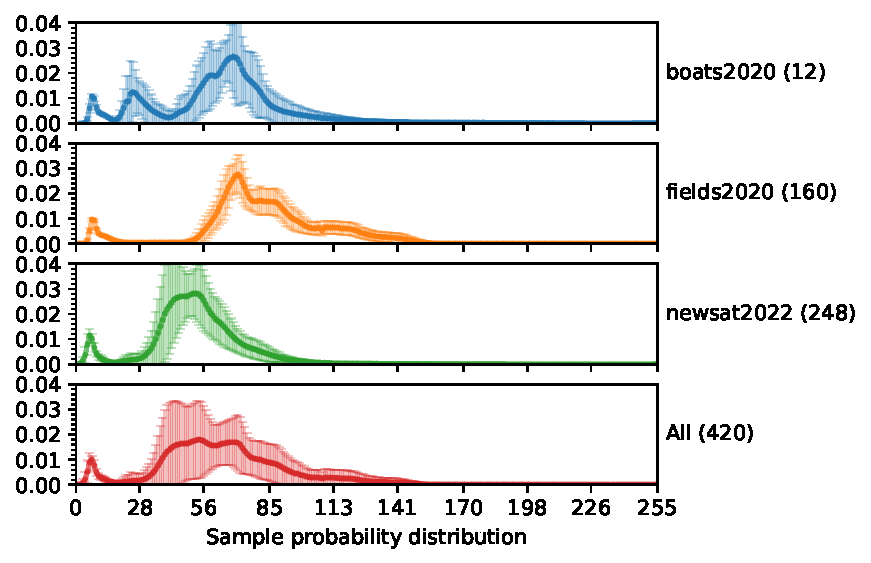
\includegraphics[width=\linewidth]{./plots/dataset_analysis/DictNumericAnalyzer-sample_distribution-line-groupby__corpus.pdf}
\end{center}
\caption{Average sample value distribution for the different test corpora and for all images.}
\label{fig:sample_distribution}
\end{figure}

\begin{figure}[h]
\begin{center}
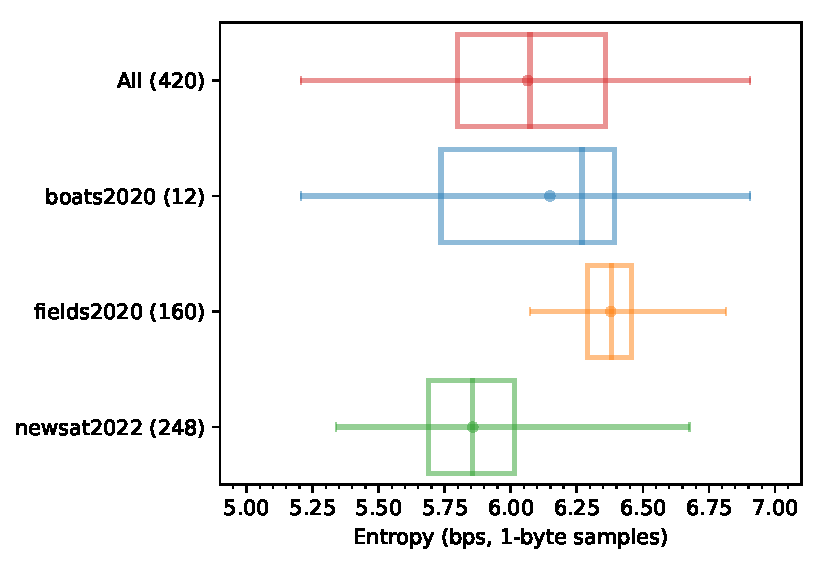
\includegraphics[width=0.75\linewidth]{./plots/dataset_analysis/ScalarNumericAnalyzer-entropy_1B_bps-boxplot-groupby__corpus.pdf}
\end{center}
\caption{Zero-order entropies. Horizontal bars indicate the minimum and maximum values, vertical bars the 25\%, 50\% and 75\% quartiles, and round dots the mean values.}
\label{fig:entropy}
\end{figure}

\begin{figure}[h]
\begin{center}
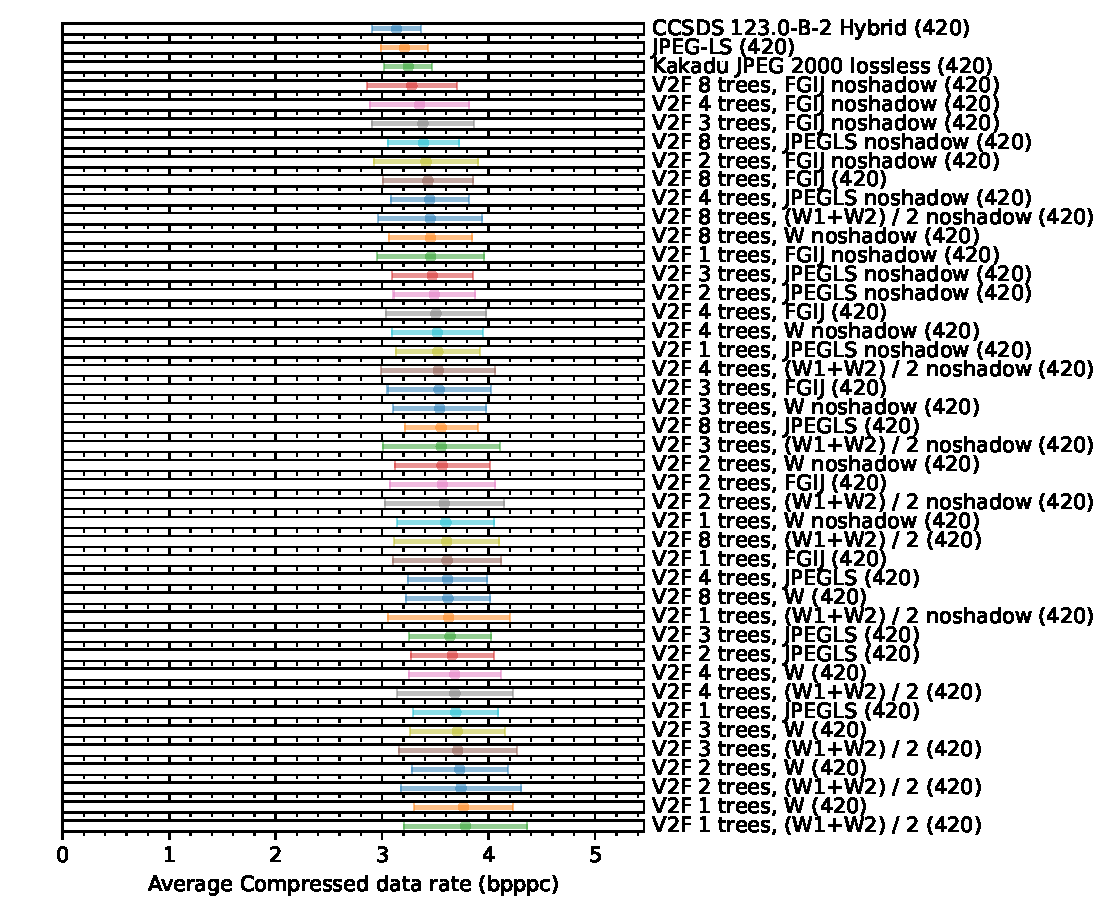
\includegraphics[width=\linewidth]{./plots/lossless/ScalarNumericAnalyzer-bpppc-histogram-groupby__family_label.pdf}
\end{center}
\caption{Average compressed data rates and $\pm$1 standard deviations for all test samples.}
\label{fig:lossless_bpppc}
\end{figure}

\begin{figure}[h]
\begin{center}
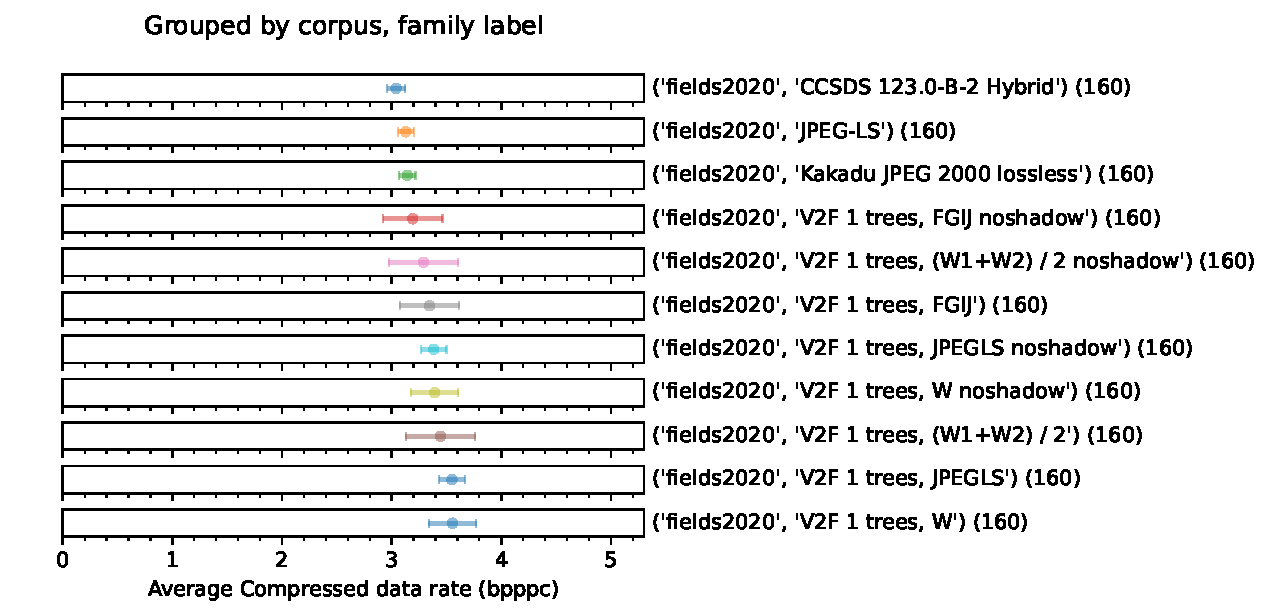
\includegraphics[width=0.9\linewidth]{./plots/lossless/fields_bpppc_histogram.pdf}
\end{center}
\caption{Average compressed data rates and $\pm$1 standard deviations for the \textit{fields2020} dataset.}
\label{fig:lossless_bpppc_fields}
\end{figure}

\begin{figure}[h]
\begin{center}
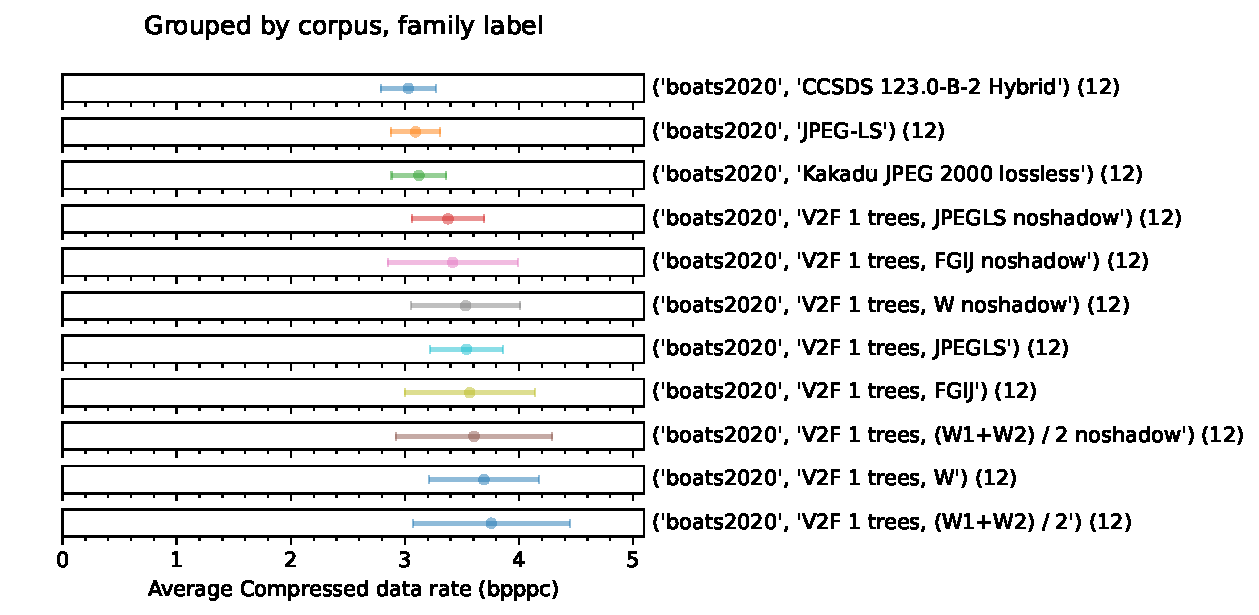
\includegraphics[width=0.9\linewidth]{./plots/lossless/boats_bpppc_histogram.pdf}
\end{center}
\caption{Average compressed data rates and $\pm$1 standard deviations for the \textit{boats2020} dataset.}
\label{fig:lossless_bpppc_boats}
\end{figure}

\begin{figure}[h]
\begin{center}
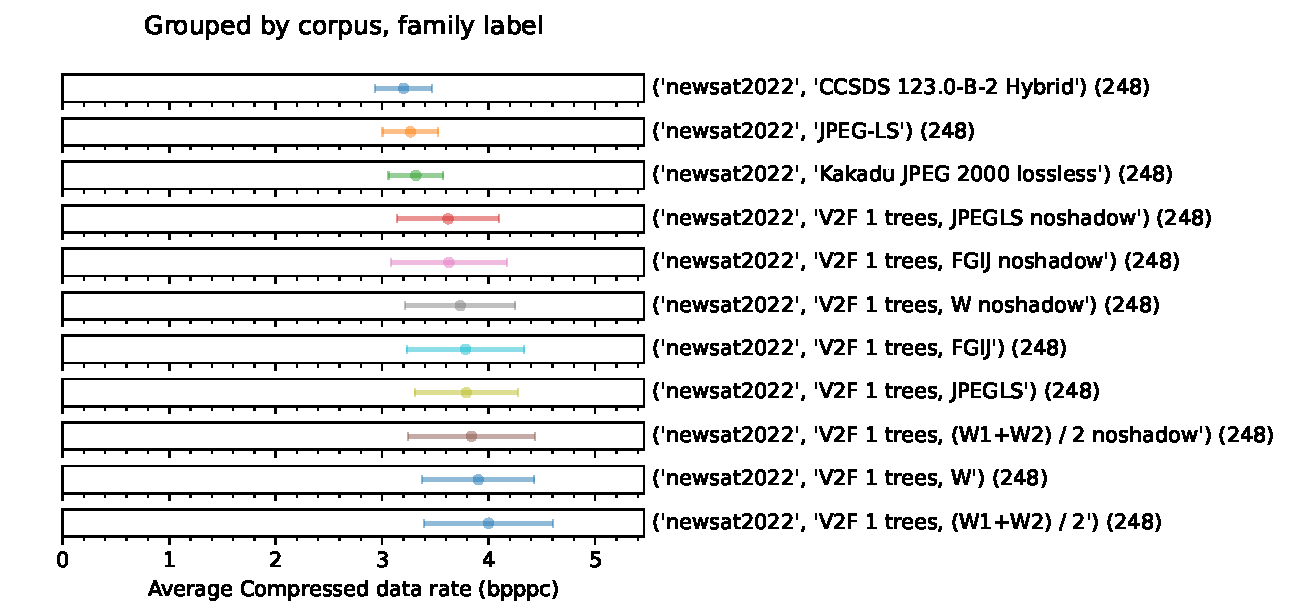
\includegraphics[width=0.9\linewidth]{./plots/lossless/newsat_bpppc_histogram.pdf}
\end{center}
\caption{Average compressed data rates and $\pm$1 standard deviations for the \textit{newsat2022} dataset.}
\label{fig:lossless_bpppc_newsat}
\end{figure}

\begin{figure}[h]
\begin{center}
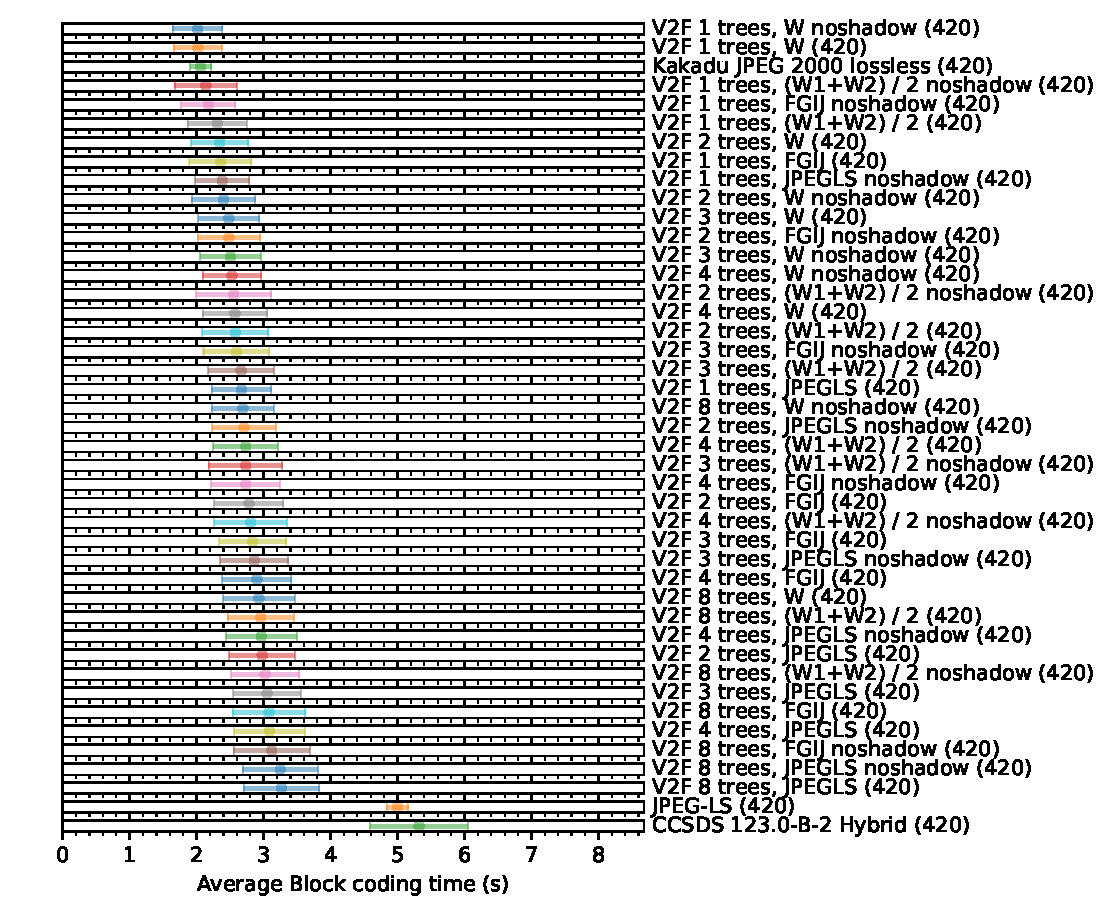
\includegraphics[width=\linewidth]{./plots/lossless/ScalarNumericAnalyzer-block_coding_time_seconds-histogram-groupby__family_label.pdf}
\end{center}
\caption{Average compression times and $\pm$1 standard deviations for all test samples.}
\label{fig:lossless_time}
\end{figure}

\begin{figure}[h]
\begin{center}
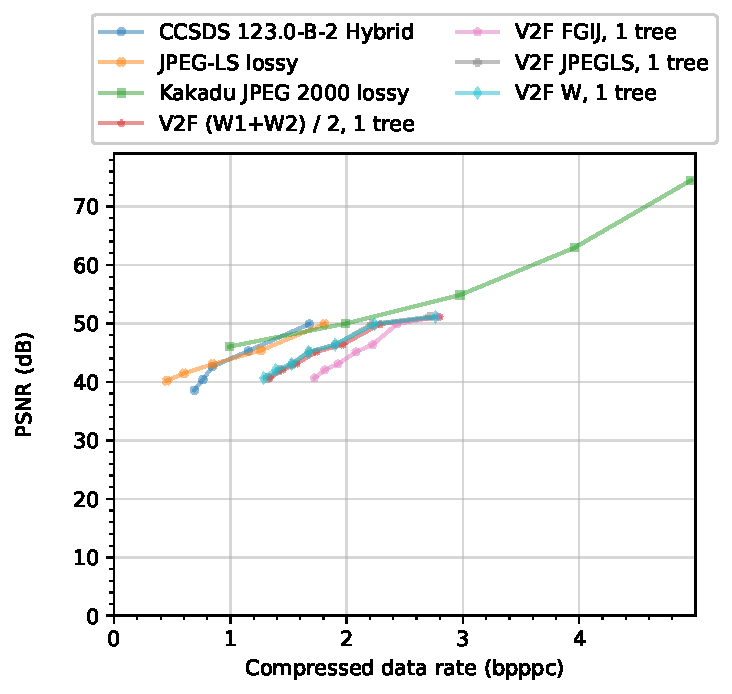
\includegraphics[width=0.6\linewidth]{./plots/lossy/TwoNumericAnalyzer-columns_bpppc__psnr_dr-line-groupby__family_label.pdf}
\end{center}
\caption{Average PSNR as a function of the compressed data rate for all test corpora.}
\label{fig:lossy_psnr}
\end{figure}

\begin{figure}[h]
\begin{center}
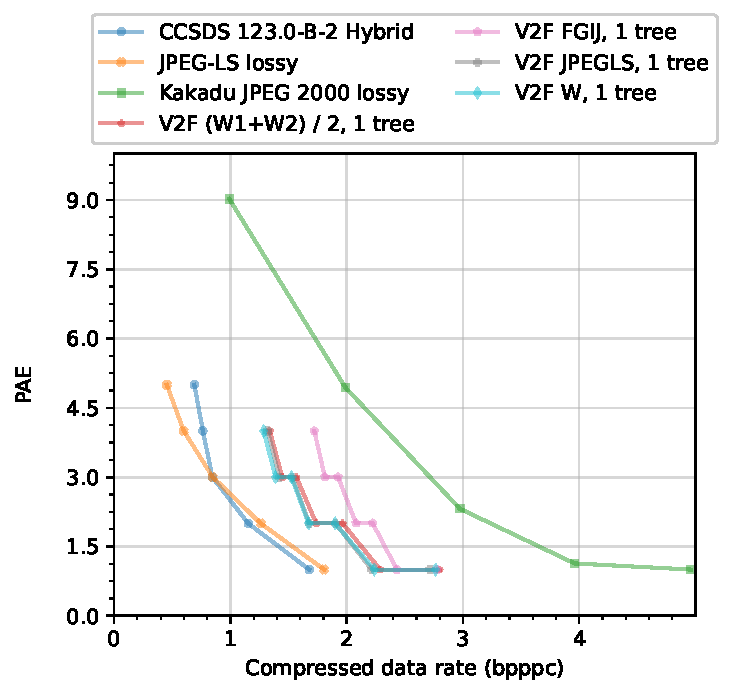
\includegraphics[width=0.6\linewidth]{./plots/lossy/TwoNumericAnalyzer-columns_bpppc__pae-line-groupby__family_label.pdf}
\end{center}
\caption{Average PAE as a function of the compressed data rate for all test corpora.}
\label{fig:lossy_pae}
\end{figure}

\begin{figure}[h]
\begin{center}
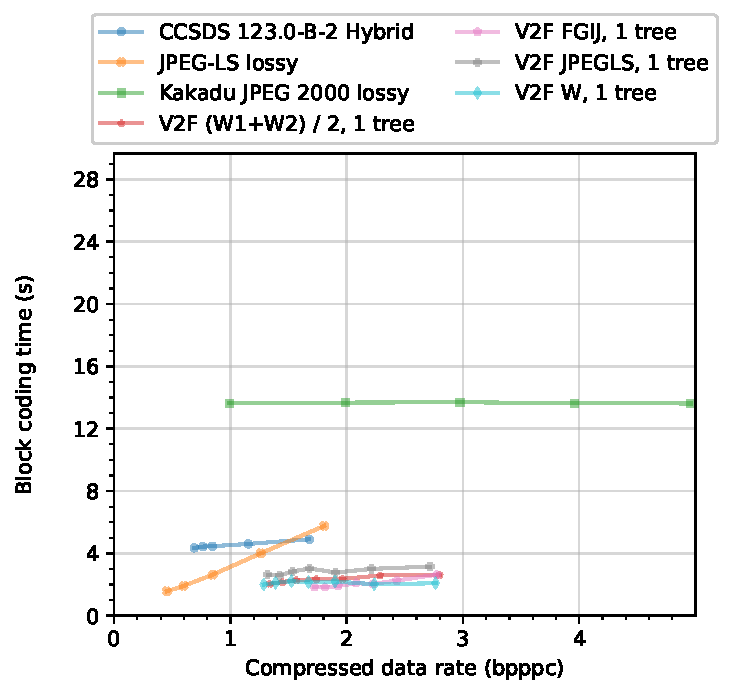
\includegraphics[width=0.6\linewidth]{./plots/lossy/TwoNumericAnalyzer-columns_bpppc__block_coding_time_seconds-line-groupby__family_label.pdf}
\end{center}
\caption{Average compression time as a function of the compressed data rate for all test corpora.}
\label{fig:lossy_time}
\end{figure}

\begin{figure}[h]
\begin{center}
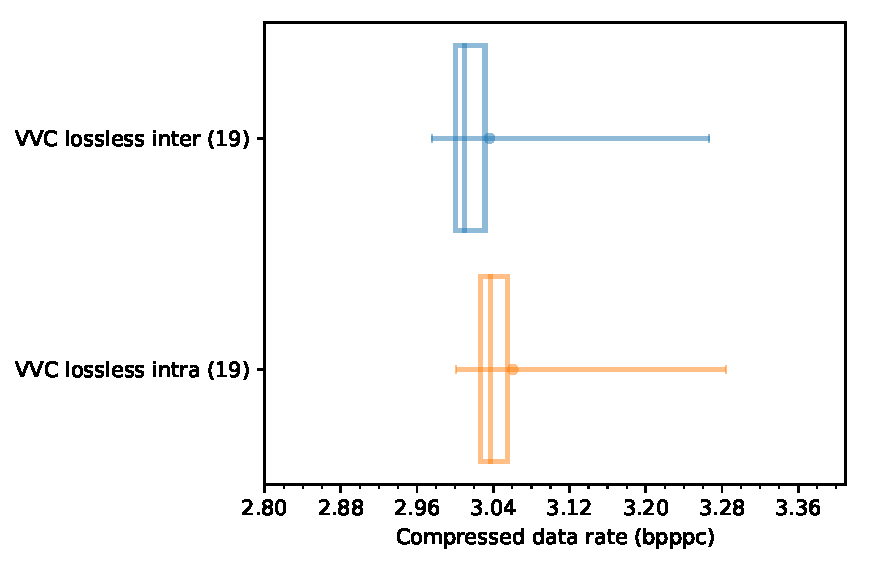
\includegraphics[width=0.6\linewidth]{./plots/extra/vvc_results.pdf}
\end{center}
\caption{Compressed data rate for VVC with (inter) and without (intra) motion compensation.
Horizontal bars indicate the minimum and maximum values, vertical bars the 25\%, 50\% and 75\% quartiles, and round dots the mean values.}
\label{fig:vvc}
\end{figure}

\begin{figure}[h]
\begin{center}
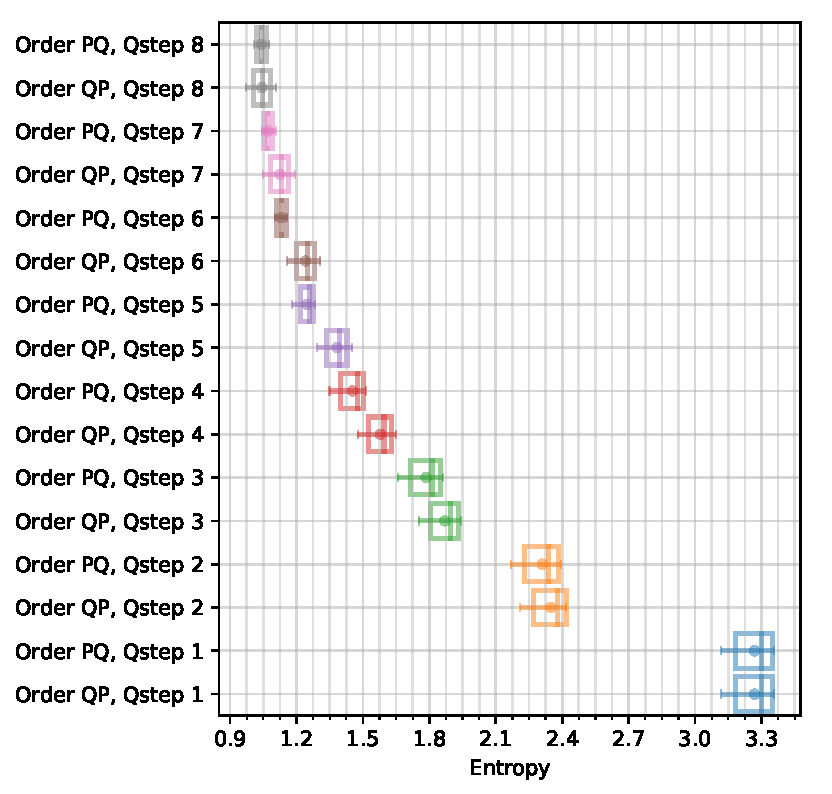
\includegraphics[width=0.7\linewidth]{./plots/extra/qp_pq_comparison.pdf}
\end{center}
\caption{Average zero-order entropy for different quantization steps for the \textit{boats2020} and \textit{fields2020} datasets.
QP denotes quantization before prediction, and PQ prediction before quantization.
Horizontal bars indicate the minimum and maximum values, vertical bars the 25\%, 50\% and 75\% quartiles, and round dots the mean values.}
\label{fig:qp_pq}
\end{figure}
% \renewcommand\refname{List of references}
% \addcontentsline{toc}{section}{List of references}
% 
% \bibliographystyle{IEEEtran}
% \bibliography{IEEEabrv,biblio}
% Use IEEEabrv if the abbreviatted journal names should be used

\end{document}
